%\documentclass[mathserif]{beamer}
\documentclass[handout]{beamer}
%\usetheme{Goettingen}
\usetheme{Warsaw}
%\usetheme{Singapore}
%\usetheme{Frankfurt}
%\usetheme{Copenhagen}
%\usetheme{Szeged}
%\usetheme{Montpellier}
%\usetheme{CambridgeUS}
%\usecolortheme{}
%\setbeamercovered{transparent}
\usepackage[english, activeacute]{babel}
\usepackage[utf8]{inputenc}
\usepackage{amsmath, amssymb}
\usepackage{dsfont}
\usepackage{graphics}
\usepackage{cases}
\usepackage{graphicx}
\usepackage{pgf}
\usepackage{epsfig}
\usepackage{amssymb}
\usepackage{multirow}	
\usepackage{amstext}
\usepackage[ruled,vlined,lined]{algorithm2e}
\usepackage{amsmath}
\usepackage{epic}
\usepackage{epsfig}
\usepackage{fontenc}
\usepackage{framed,color}
\usepackage{palatino, url, multicol}
\usepackage{listings}
%\algsetup{indent=2em}


\vspace{-0.5cm}
\title{Directed Graphical Models}
\vspace{-0.5cm}
\author[Felipe Bravo Márquez]{\footnotesize
%\author{\footnotesize  
 \textcolor[rgb]{0.00,0.00,1.00}{Felipe José Bravo Márquez}} 
\date{ \today }




\begin{document}
\begin{frame}
\titlepage


\end{frame}


%%%%%%%%%%%%%%%%%%%%%%%%%%%


\begin{frame}{Directed Graphical Models}
\scriptsize{
\begin{itemize}
\item Probabilistic graphical models (PGMs) are a rich framework for encoding probability distributions over complex domains  \cite{koller2009probabilistic}.

\item In this class we will focus on directed graphical models (DGMs), which are one type of PGM.

\item Directed graphical models (DGMs) are a family of probability distributions that admit a compact parametrization that can be naturally described using a directed graph.

\item DGMs are also known as Bayesian networks.

\item Statistical inference for DGMs can be performed using frequentist or Bayesian methods, so it is misleading to call them Bayesian networks \cite{wasserman2013all}.



 
\end{itemize}



} 

\end{frame}


\begin{frame}{Directed Acyclic Graphs (DAGs)}
\scriptsize{
\begin{itemize}
\item A directed graph consists of a set of nodes with arrows between some nodes.


\item Graphs are useful for representing independence relations between variables.

\item More formally, a directed graph G consists of a set of vertices V and an edge set E of ordered pairs of
vertices.

\item For our purposes, each vertex corresponds to a random variable. 

\item If $(Y, X) \in E$  then there is an arrow pointing from Y to X. 

\begin{figure}[h!]
	\centering
	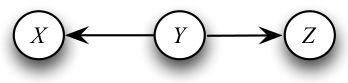
\includegraphics[scale=0.5]{pics/dag1.png}
	\caption{A directed graph with vertices $V = \{X, Y, Z\}$ and edges $E = \{(Y, X), (Y, Z)\}$.}
	\end{figure} 


 
\end{itemize}



} 

\end{frame}



\begin{frame}{Directed Acyclic Graphs (DAGs)}
\scriptsize{
\begin{itemize}
\item If an arrow connects two variables X and Y (in either direction) we say that X and Y are adjacent.


\item If there is an arrow from X to Y then X is a parent of Y and Y is a child of X.

\item The set of all parents of X is denoted by $\pi_{X}$ or $\pi(X)$.

\item A directed path between two variables is a set of arrows all pointing in the same direction linking one variable to the
other such as the chain shown below:

\begin{figure}[h!]
	\centering
	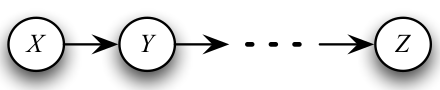
\includegraphics[scale=0.5]{pics/dag2.png}
	\caption{A chain graph with a directed path.}
	\end{figure} 

\item X is an ancestor of Y if there is a directed path from X to Y (or X = Y ).

\item We also say that Y is a descendant of X.
 
\end{itemize}



} 

\end{frame}

\begin{frame}{Directed Acyclic Graphs (DAGs)}
\scriptsize{
\begin{itemize}
\item A directed path that starts and ends at the same variable is called a cycle.

\item A directed graph is acyclic if it has no cycles. 

\item In this case we say that the graph is a directed
acyclic graph or DAG. 


\begin{figure}[h!]
	\centering
	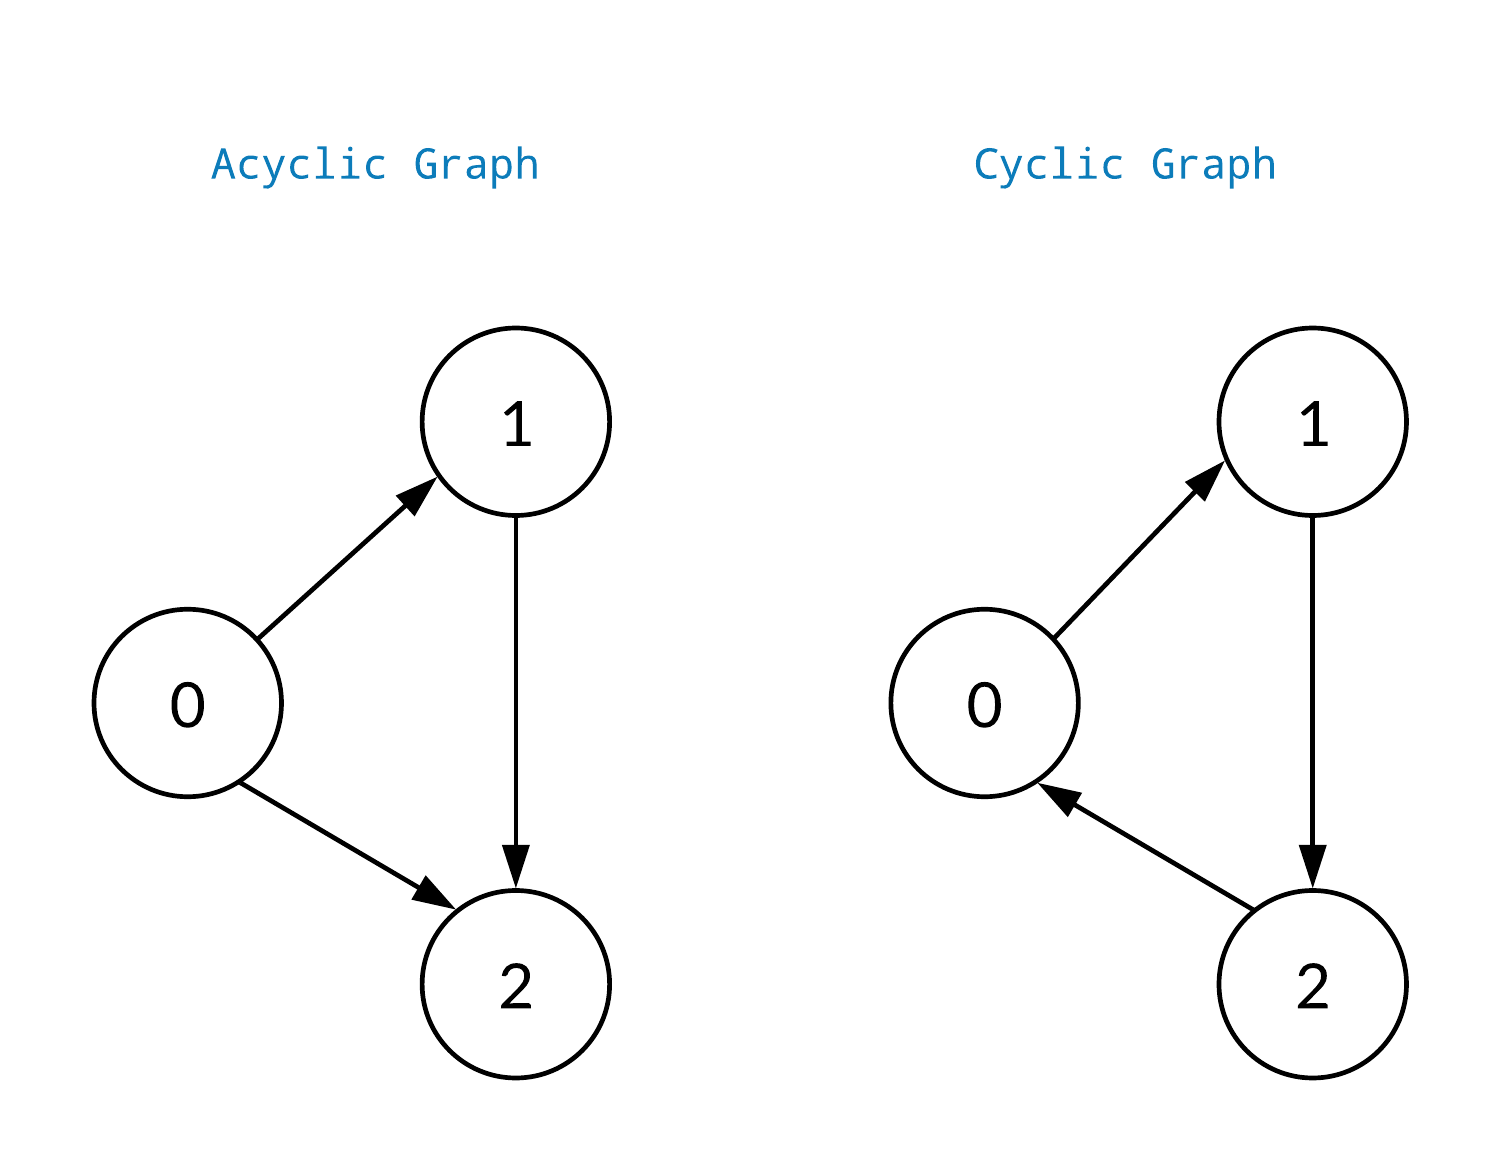
\includegraphics[scale=0.12]{pics/cycle.png}
	\end{figure} 



\item From now on, we only deal with directed acyclic graphs since it is very difficult to provide a coherent probability semantics over graphs with directed cycles.
 
\end{itemize}



} 

\end{frame}


\begin{frame}{Probability and DAGs}
\scriptsize{
\begin{itemize}
\item Let $G$ be a DAG with vertices $V = (X_1 , \dots , X_d )$. 

\item If $P$ is a distribution for $V$ with probability function $f(x)$ (density or masss), we say that $G$ represents $P$ , if

\begin{displaymath}
 f(x) = \prod_{j=1}^d f(x_j| \pi_{x_j})
\end{displaymath}

where $\pi_{x_j}$ is the set of parent nodes of $X_j$

\item The next figute shows a DAG with four variables.

\begin{figure}[h!]
	\centering
	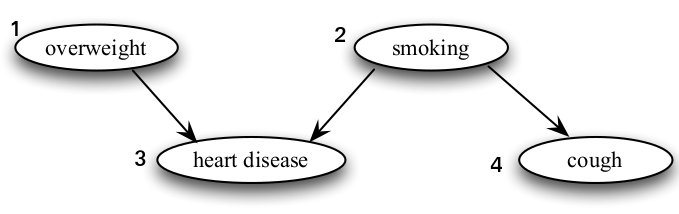
\includegraphics[scale=0.3]{pics/dag3.png}
	\end{figure} 



\item The probability function takes the following decomposition:

\item $f($overweight, smoking, heart disease, cough$) =$ \\    $f($overweight$) \times f($smoking$) \times f($heart, disease$|$ overweight, smoking$) \times f($cough$|$smoking$)$. 



\end{itemize}



} 

\end{frame}







\begin{frame}{Conditional Independence}
\scriptsize{
\begin{itemize}
\item Let $X$, $Y$ and $Z$ be random variables. 

\item $X$ and $Y$ are conditionally independent given $Z$, written $X \perp Y | Z$, if:

\begin{displaymath}
f(x, y|z) = f(x|z)f(y|z) 
\end{displaymath}


for all x, y and z.

\item Notice that $f$ can be either a density function for continous random variables or a probability mass function for discrete random variables.
 
\item Intuitively, this means that, once you know $Z$, $Y$ provides no extra information about $X$. 
 
\end{itemize}



} 

\end{frame}


\begin{frame}{D-separation}
\scriptsize{
\begin{itemize}
\item sdsad

 
\end{itemize}



} 

\end{frame}


\begin{frame}{Conclusions}
\scriptsize{

\begin{itemize}
\item Blabla
\end{itemize}


} 
\end{frame}


%%%%%%%%%%%%%%%%%%%%%%%%%%%
\begin{frame}[allowframebreaks]\scriptsize
\frametitle{References}
\bibliography{bio}
\bibliographystyle{apalike}
%\bibliographystyle{flexbib}
\end{frame}  









%%%%%%%%%%%%%%%%%%%%%%%%%%%

\end{document}
